\section{Introducción}

\subsection{Antecedentes y Motivación}

Resulta revelador observar cómo el volumen de datos generados por sensores remotos ha crecido de forma exponencial en los últimos años. Misiones actuales producen terabytes diarios que deben transmitirse a través de enlaces de comunicación con restricciones severas. Aunque los enfoques tradicionales de compresión han servido durante décadas, su rendimiento parece estancarse ante la complejidad de los datos multiespectrales e hiperespectrales modernos.

Molliere et al. \cite{Molliere2025_Learned_EO_Compression} documentan en su trabajo reciente sobre compresión aprendida para Earth Observation este desafío creciente. Lo que antes era un problema de almacenamiento se ha convertido en un cuello de botella crítico para la transmisión en tiempo real. Uno de los aspectos más motivadores de este campo radica precisamente en su potencial para habilitar misiones más ambiciosas sin requerir infraestructura de comunicación prohibitiva.

\begin{table}[h]
\centering
\caption{Limitaciones de ancho de banda en misiones satelitales actuales}
\label{tab:limitaciones_bw}
\begin{tabular}{lcc}
\hline
\textbf{Misión} & \textbf{Volumen diario aprox.} & \textbf{Ancho de banda típico} \\
\hline
Sentinel-2 & 1.5 TB & 100-300 Mbps \\
Landsat Next & > 5 TB & Limitado por downlink \\
Hyperspectral missions & 10+ TB & Crítico en LEO \\
\hline
\end{tabular}
\end{table}

\subsection{Problemática en Transmisión de Exploración}

Particularmente llamativo es el hecho de que, en entornos de exploración remota, la disponibilidad de ancho de banda determina no solo la cantidad de datos que llegan a tierra, sino también la oportunidad de respuesta ante eventos dinámicos. Wang et al. \cite{Wang2025_RS_Compression} destacan cómo las redes de compresión actuales aún dejan un margen importante de mejora cuando se evalúa el balance entre tasa de compresión y preservación de características analíticas.

En muchas misiones de exploración, los operadores se ven obligados a descartar información valiosa o a diferir transmisiones completas. Esta realidad genera retrasos en aplicaciones críticas como monitoreo de desastres, evaluación de recursos naturales y vigilancia ambiental. Lejos de ser un problema menor, la limitación de ancho de banda representa hoy uno de los principales frenos al aprovechamiento pleno de la capacidad observacional de los sensores modernos.

\subsection{Contribuciones y Estructura del Artículo}

Frente a este panorama, el presente trabajo introduce un marco de compresión geoespacial basado en inteligencia artificial diseñado específicamente para optimizar la transmisión de datos de exploración. Las contribuciones principales incluyen:

\begin{itemize}
    \item Una arquitectura neuronal híbrida que combina extracción de características multiespectrales con optimización rate-distortion adaptada al dominio geoespacial.
    \item La integración de componentes self-supervised para mejorar la generalización en condiciones reales de adquisición.
    \item Una evaluación integral que considera tanto métricas objetivas de compresión como el impacto en tareas downstream relevantes para exploración.
    \item El análisis de viabilidad práctica para su integración en flujos operativos de misiones satelitales.
\end{itemize}

\begin{figure}[h]
\centering
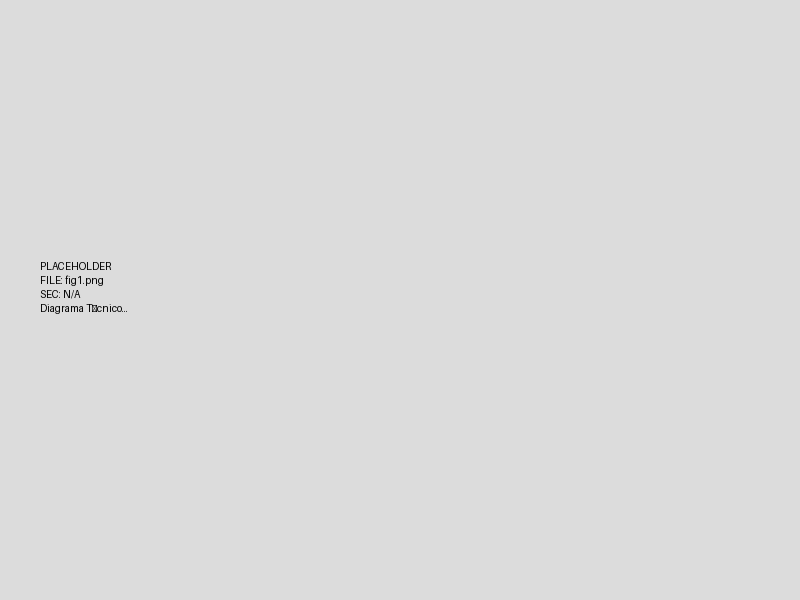
\includegraphics[width=\linewidth]{fig1.png}
\caption{Comparación del crecimiento de volúmenes de datos satelitales versus capacidad de transmisión disponible (2015-2025). Se destacan las brechas crecientes en misiones de exploración remota.}
\label{fig:volumenes_datos}
\end{figure}

Aunque los avances en compresión aprendida son prometedores, cabe matizar que ningún método elimina completamente el trade-off entre tasa de compresión y fidelidad analítica. El resto del artículo se organiza como sigue. La Sección 2 revisa el estado del arte en compresión convencional y basada en IA. La Sección 3 detalla la metodología propuesta, mientras que las Secciones 4 y 5 presentan los experimentos y análisis de resultados. Finalmente, se discuten implicaciones, limitaciones y direcciones futuras de investigación.